\newpage
\subsection{Đăng nhập và Xác thực đa yếu tố (MFA)}
\subsubsection*{Mục tiêu}
Cho phép người dùng đăng nhập bằng cách nhập \codefile{email} và \codefile{passphrase}. Nếu thông tin hợp lệ, hệ thống sẽ yêu cầu xác minh OTP qua email hoặc mã TOTP (Google Authenticator). Hệ thống hỗ trợ các biện pháp bảo mật nâng cao:
\begin{itemize}
    \item Bảo vệ bằng xác thực 2 yếu tố
    \item Tự động khóa tài khoản 5 phút sau 5 lần đăng nhập sai
    \item Cho phép admin khóa tài khoản thủ công
    \item Ghi log toàn bộ hành vi đăng nhập
\end{itemize}
\subsubsection*{Giao diện}
Giao diện \codefile{/auth/login} là form HTML bao gồm 2 trường:
\begin{itemize}
    \item Email
    \item Passphrase
\end{itemize}
\begin{figure}[H]
\centering
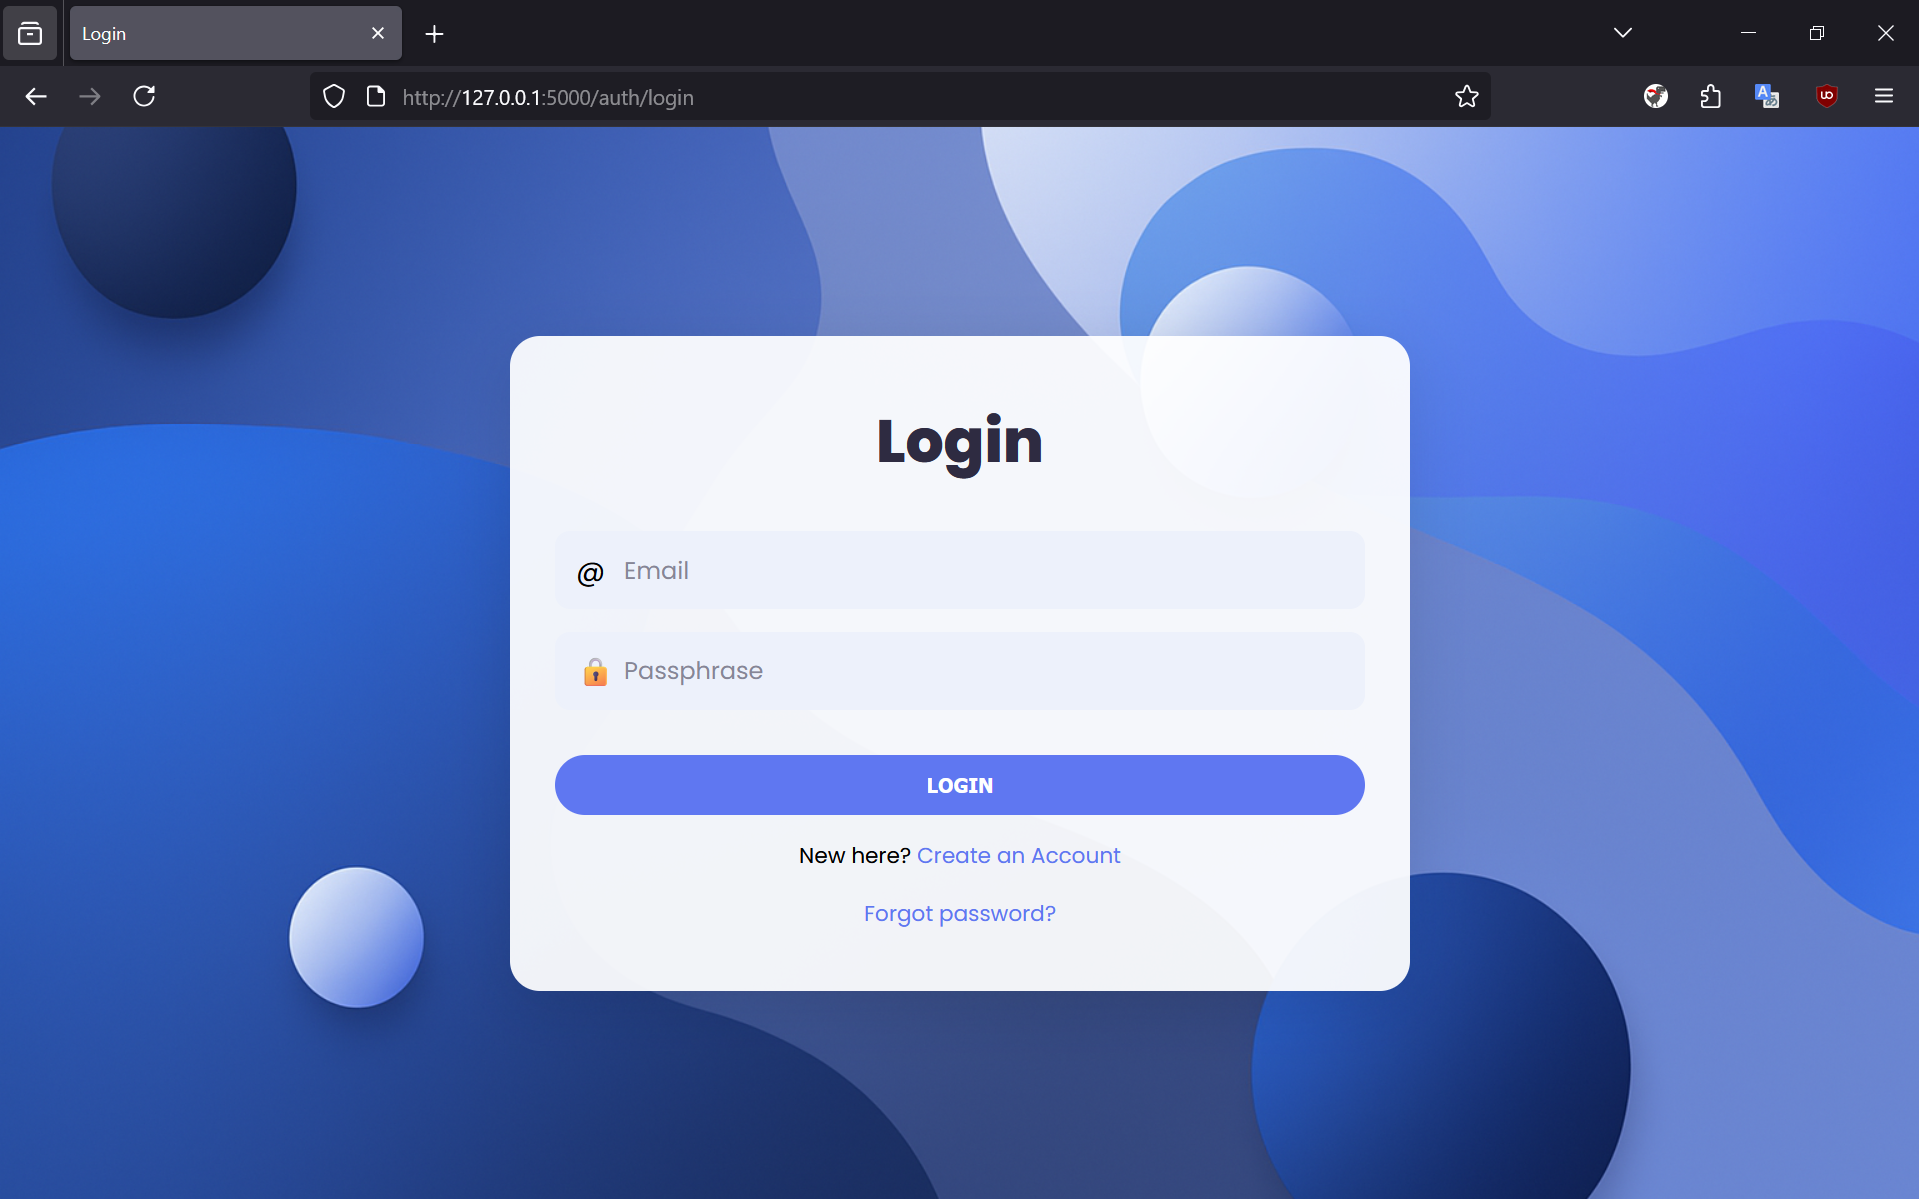
\includegraphics[scale=0.34]{img/login.png}
\caption{Giao diện Login}
\label{fig:login_ui}
\end{figure}

Sau khi đăng nhập thành công, người dùng được chuyển đến \codefile{/auth/verify} để xác thực MFA bằng 1 trong 2 phương thức:
\begin{enumerate}
    \item OTP gửi qua email (mặc định)
    \begin{figure}[H]
    \centering
    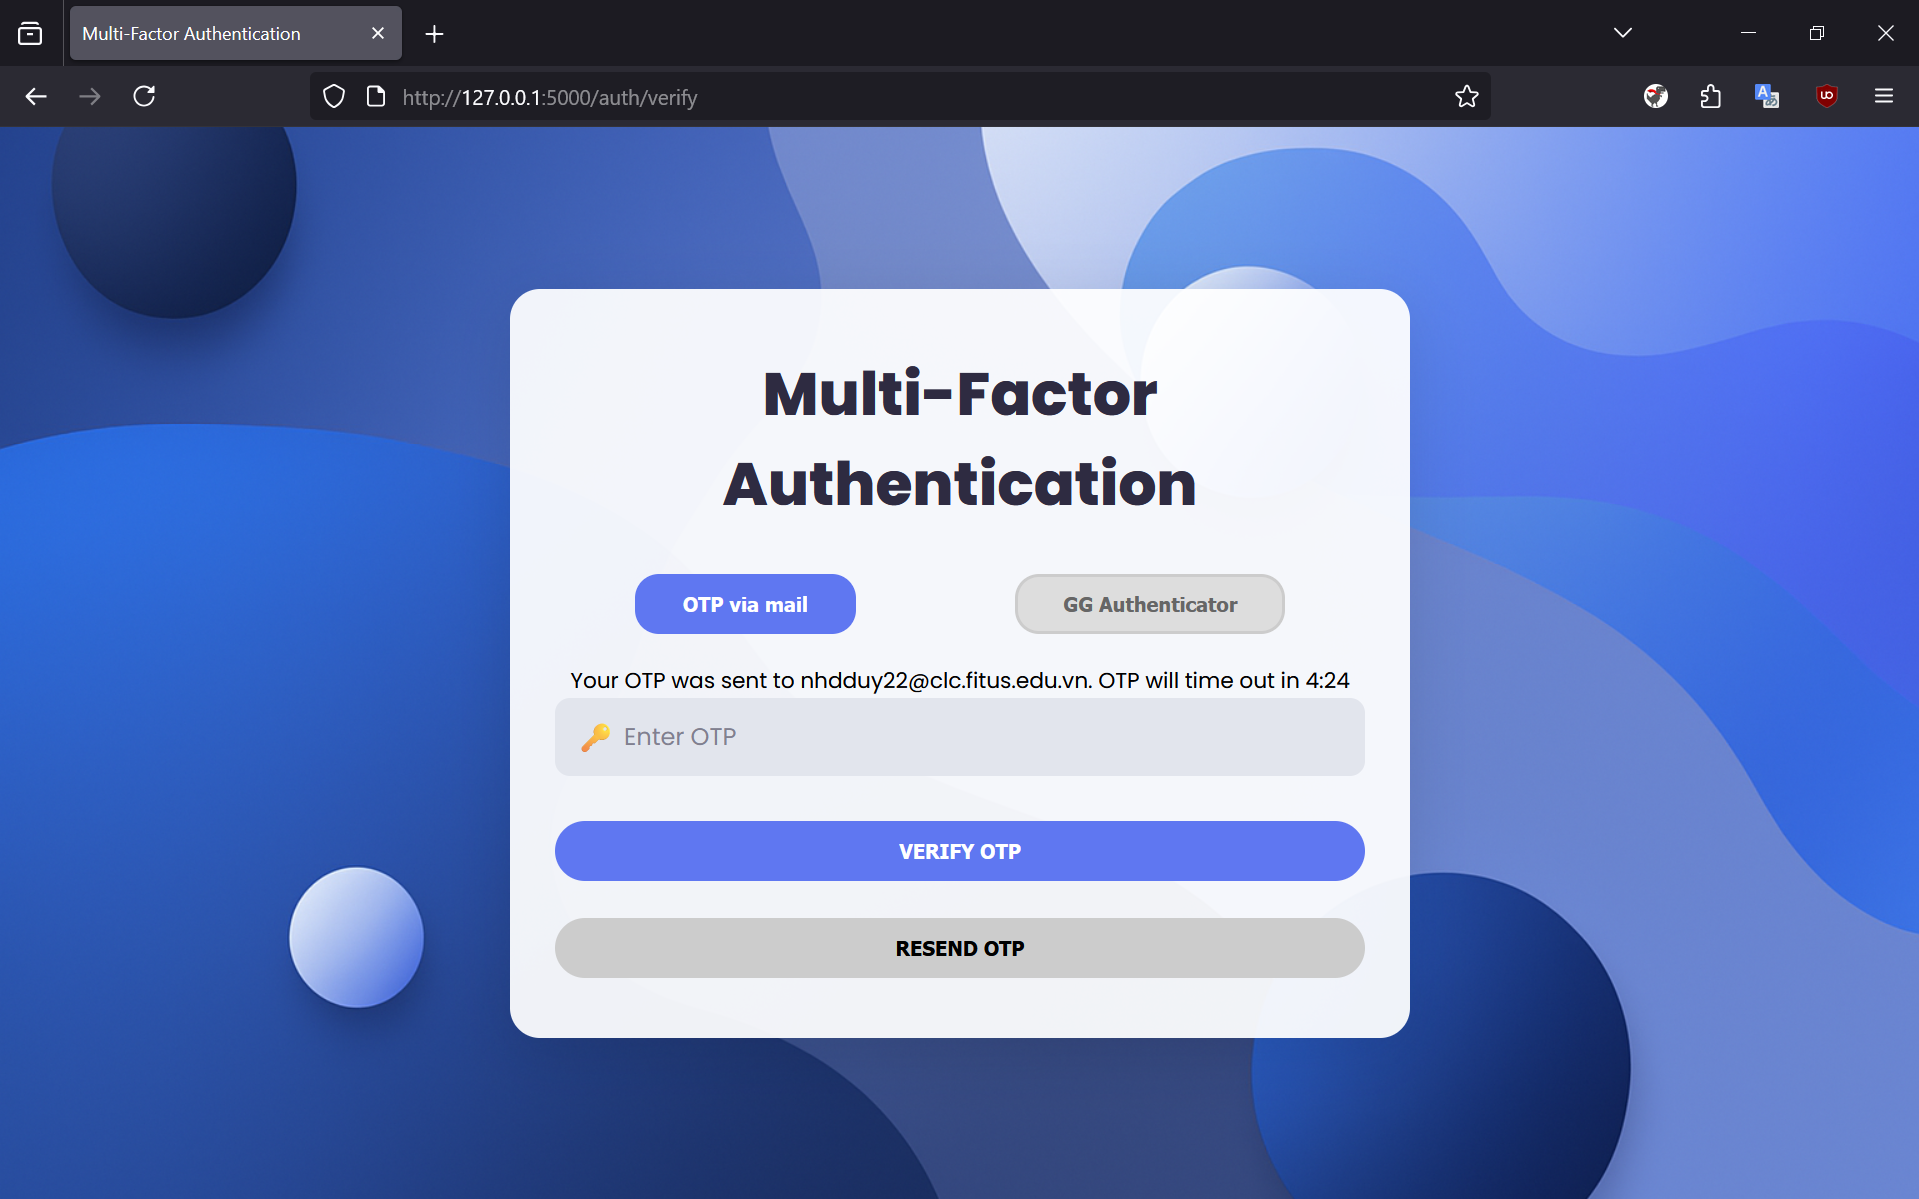
\includegraphics[scale=0.28]{img/MFA-OTP.png}
    \caption{Xác thực bằng OTP gửi qua mail}
    \label{fig:opt_ui}
    \end{figure}
    
    \item Mã TOTP (QR code cho Google Authenticator)
    \begin{figure}[H]
    \centering
    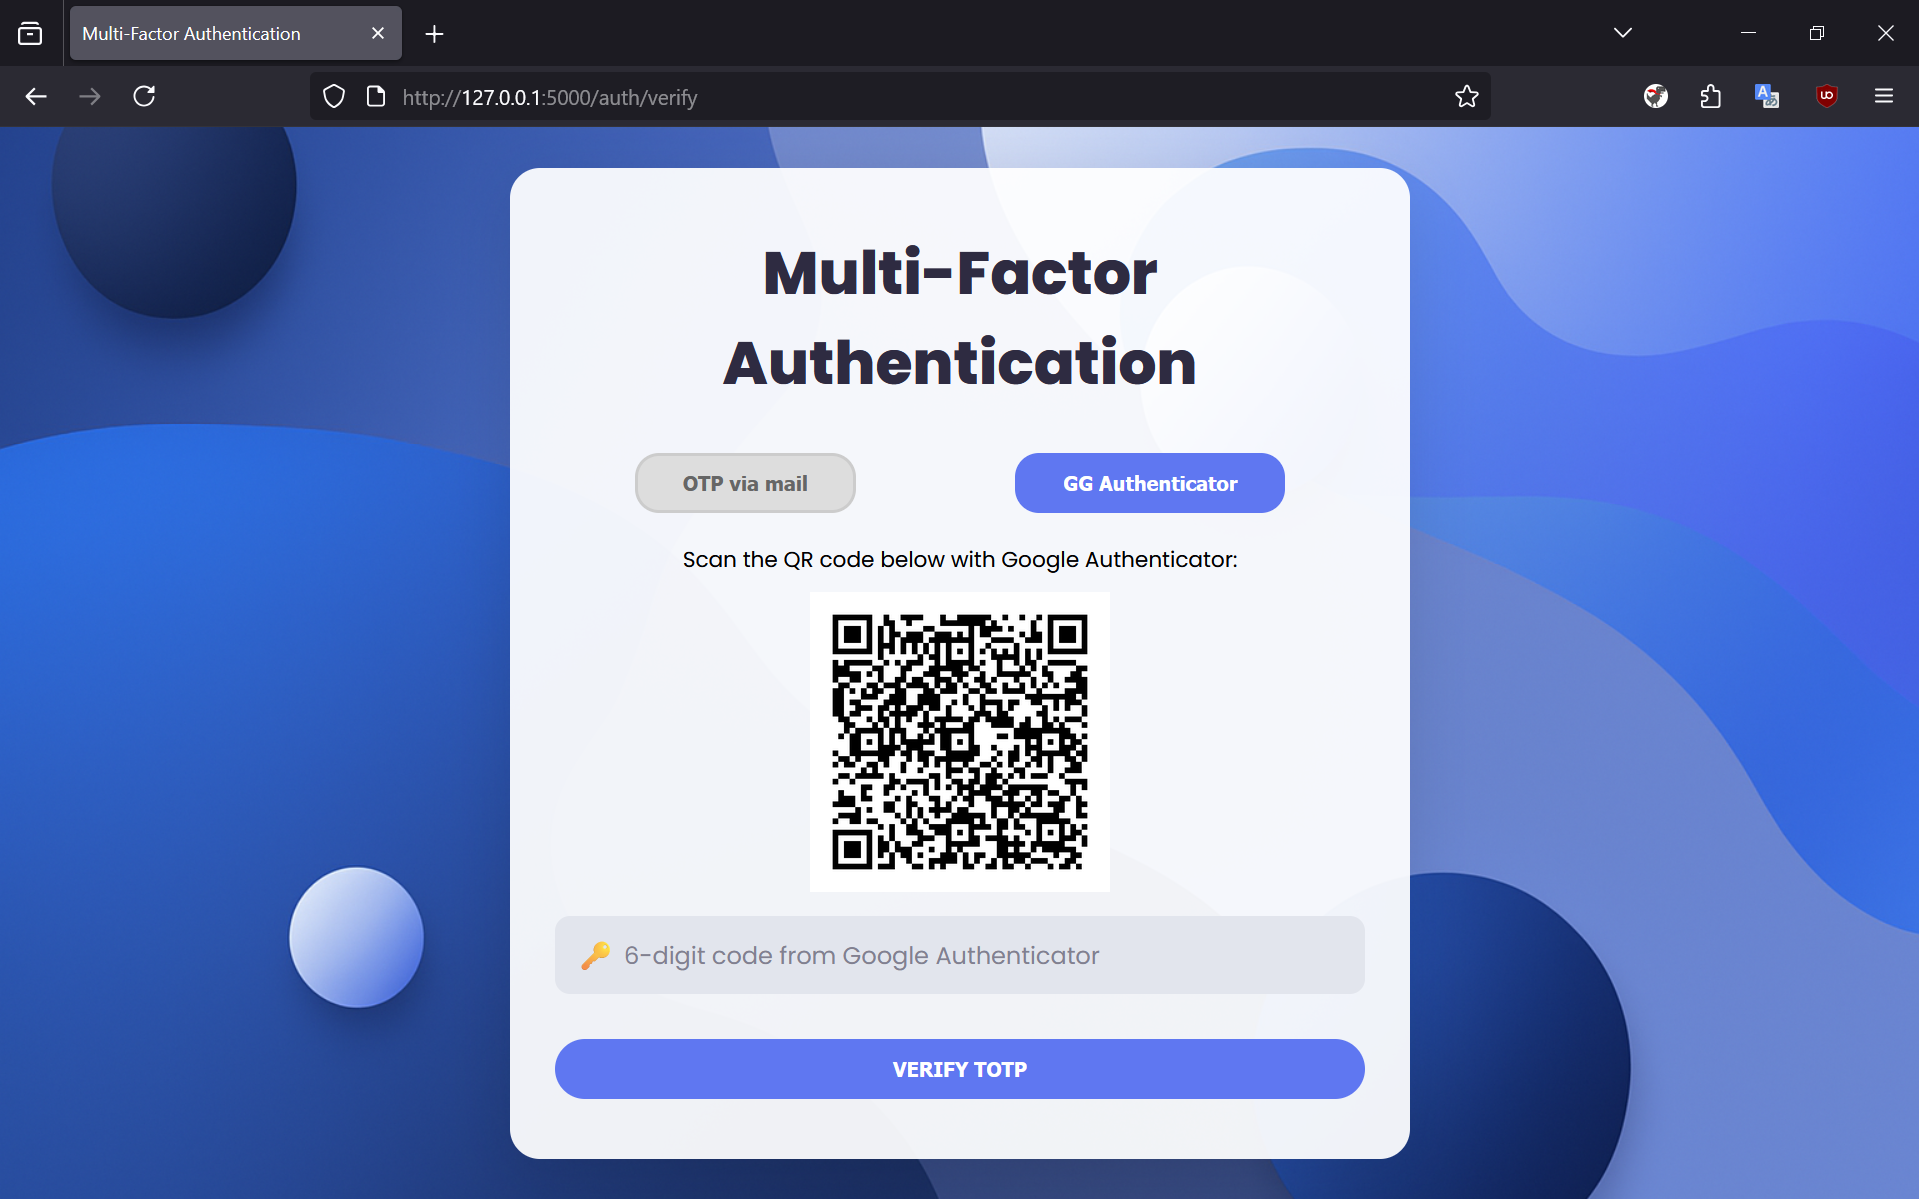
\includegraphics[scale=0.28]{img/MFA-TOTP.png}
    \caption{Xác thực bằng TOTP qua QR code}
    \label{fig:totp_ui}
    \end{figure}
\end{enumerate}

\subsubsection*{Quy trình thực hiện}
\begin{enumerate}
    \item Người dùng submit form \codefile{/auth/login} với \codefile{email} và \codefile{passphrase}.
    \item Flask gọi hàm \codefile{process\_login(email, passphrase) )} trong \codefile{logic.py}
    \item Chương trình thực hiện:
    \begin{itemize}
        \item Kiểm tra người dùng tồn tại hay không.
        \item So sánh \codefile{hash(passphrase + salt)}.
        \item Nếu sai, tăng \codefile{failed\_attempts} và cập nhật \codefile{last\_failed\_login}. 
        \item Nếu sai hơn 5 lần trong 2 phút $\rightarrow$ Gán \codefile{is\_locked = 1}, trả về trạng thái \textbf{locked}.
        \item Nếu tài khoản bị khóa bởi admin (\codefile{last\_failed\_login = null} và \codefile{is\_locked = 1}) $\rightarrow$ trả về \textbf{locked by admin}.
        \item Nếu các thông tin đăng nhập đúng $\rightarrow$ Reset \codefile{failed\_attempts}, ghi log, chuyển đến bước xác thực MFA.
    \end{itemize}
    \item Người dùng được chuyển đến \codefile{/auth/verify}, chọn xác thực OTP qua email hoặc quét QR TOTP (mặc định là gửi OTP qua email đã đăng ký).
    \item Nếu chọn OTP:
    \begin{itemize}
        \item Gọi \codefile{generate\_and\_send\_otp(email)} $\rightarrow$ sinh mã 6 chữ số, gửi qua email, lưu DB kèm thời gian hết hạn.
        \begin{figure}[H]
        \centering
        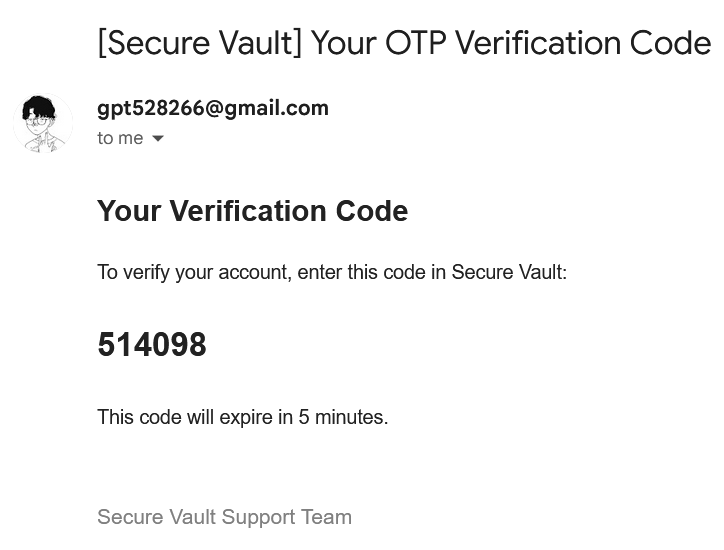
\includegraphics[scale=0.34]{img/mail-otp.png}
        \caption{Cấu trúc mail}
        \label{fig:mail_recovery_ui}
        \end{figure}
        \item Kiểm tra bằng \codefile{verify\_otp\_code(email, input\_code)}.
    \end{itemize}
    \item Nếu chọn TOTP:
    \begin{itemize}
        \item Sinh mã QR từ \codefile{generate\_qr\_code(email)} $\rightarrow$ dùng cho ứng dụng Google Authenticator.
        \item Kiểm tra bằng \codefile{verify\_totp\_code(email, input\_code)}.
    \end{itemize}
    \item Nếu đúng $\rightarrow$ Lưu \codefile{session['user\_id]} và chuyển đến \codefile{auth/dashboard}
\end{enumerate}

\subsubsection*{Chi tiết kỹ thuật và thư viện bảo mật}
\textbf{1. Hashing passphrase với Salt}

Thư viện: \codefile{hashlib} 

Kỹ thuật:
\begin{itemize}
    \item Salt đã được sinh bằng \codefile{os.urandom(16).hex()} $\rightarrow$.
    \item Kiểm tra \codefile{passphrase} được người dùng nhập vào sau khi hash có giống với chuỗi được lưu trong DB hay không.
\end{itemize}

\textbf{2. Gửi mã OTP qua email}

Thư viện: \codefile{random, datetime, smtplib, email} 

Kỹ thuật:
\begin{itemize}
    \item Sinh mã 6 chữ số ngẫu nhiên.
    \item Lưu \codefile{expires\_at = now + 5 minutes}
    \item Dùng \codefile{email.mime.text} và \codefile{email.mime.multipart} để format tin nhắn gửi email.
    \item Tạo tài khoản gmail đã xác thực 2 yếu tố và tiến hành tạo \codefile{app password} và lưu vào \codefile{.env} với cấu trúc như sau
\begin{lstlisting}
SMTP_USER=<sender mail>
SMTP_PASS=<app password>
\end{lstlisting}
    \item OTP được tạo sẽ lưu vào DB và gửi bằng SMTP $\rightarrow$ người dùng cần kiểm tra email để nhận OTP.
    \item Người dùng nhập mã OTP $\rightarrow$ Server sẽ lấy bản \codefile{otp\_code} mới nhất và kiểm tra xem mã có đúng và còn hạn hay không $\rightarrow$ Nếu hợp lệ, người dùng xác thực thành công
\end{itemize}

\textbf{3. TOTP}

Thư viện: \codefile{pyotp, qrcode, base64} 

Kỹ thuật:
\begin{itemize}
    \item Mỗi tài khoản có một \codefile{mfa\_secret} (chuỗi \codefile{base32}) sinh ngẫu nhiên và được lưu trong bảng \codefile{users}.
    \item Dùng \codefile{pyotp.totp.TOTP(mfa\_secret).provisioning\_uri()} để tạo ra URI định dạng chuẩn TOTP.
    \item Sinh ảnh QR code từ URI trên.
    \item Người dùng sử dụng Google Authenticator để quét mã trên.
    \item Người dùng nhập 6 số do app tạo ra mỗi 30 giây.
    \item Server sẽ dùng lại \codefile{mfa\_secret} từ DB để sinh lại mã đúng tại thời điểm đó. Nếu mã số giống nhau thì người dùng xác thực thành công.
\end{itemize}